\documentclass[11pt,a4paper]{article}
\usepackage{fontspec}
\usepackage{xeCJK}
\setCJKmainfont[AutoFakeBold=2]{SimSun}
\setCJKsansfont{Microsoft YaHei}
\setCJKmonofont{SimSun}
\usepackage[margin=1.85cm]{geometry}
\usepackage{xcolor}
\usepackage{tikz}
\usetikzlibrary{arrows.meta,positioning,calc}
\usepackage{booktabs}
\usepackage{tabularx}
\usepackage{array}
\usepackage{enumitem}
\usepackage{fancyhdr}
\usepackage{hyperref}
\usepackage{listings}
\usepackage{amsmath}
\usepackage{amssymb}

\definecolor{navy}{HTML}{17365D}
\definecolor{blue}{HTML}{2F75B5}
\definecolor{lightblue}{HTML}{EEF5FA}
\definecolor{green}{HTML}{548235}
\definecolor{lightgreen}{HTML}{EEF6EA}
\definecolor{orange}{HTML}{C55A11}
\definecolor{lightorange}{HTML}{FFF3E8}
\definecolor{red}{HTML}{A61B1B}
\definecolor{purple}{HTML}{7030A0}
\definecolor{gray}{HTML}{5B6573}
\definecolor{lightgray}{HTML}{F4F6F8}

\hypersetup{colorlinks=true,linkcolor=blue,urlcolor=blue}
\setlength{\parindent}{0pt}
\setlength{\parskip}{4pt}
\setlist[itemize]{leftmargin=1.5em,itemsep=2pt,topsep=3pt}
\setlist[enumerate]{leftmargin=1.7em,itemsep=2pt,topsep=3pt}
\setlength{\emergencystretch}{3em}
\sloppy

\pagestyle{fancy}
\fancyhf{}
\setlength{\headheight}{14pt}
\fancyhead[L]{\textcolor{gray}{Tri-EvoBench | Weekly Progress}}
\fancyhead[R]{\textcolor{gray}{2026-09-12}}
\fancyfoot[C]{\textcolor{gray}{\thepage}}

\newenvironment{callout}{\begin{quote}\small\color{navy}}{\end{quote}}
\newcommand{\code}[1]{\texttt{#1}}
\newcommand{\pos}[1]{\textcolor{green}{\textbf{+#1}}}
\newcommand{\negv}[1]{\textcolor{red}{\textbf{-#1}}}

\title{\vspace{-1.2cm}\textcolor{navy}{Tri-EvoBench 周度进展报告}\par\vspace{5pt}\Large 全量 Baseline 矩阵与 L2 自进化探针}
\author{项目组}
\date{2026 年 9 月 12 日}

\begin{document}
\maketitle
\thispagestyle{empty}

\begin{center}
\textcolor{gray}{Hermes、SkillOpt、Trace2Skill | L1 Arena、L2 Demo V2 | Docker 真实运行}
\end{center}

\vspace{5pt}
\begin{callout}
本周形成了两组可以直接用于后续研究的结果。第一组是三种自进化 Agent 在 L1/L2 上的全量统一矩阵，共 87 个 stream-agent 任务、1,671 个 agent-turn：L1 中 SkillOpt 以更低 token 成本取得最佳综合表现，L2 中 Hermes 的任务完成能力领先。第二组是 L2 的 reset/frozen/evolving 匹配探针：Hermes 和 SkillOpt 的 evolving 条件分别比 reset 提高 0.1441 和 0.0669 mean score，而 Trace2Skill 下降 0.0184。当前证据支持“前两种方法产生了正向迁移”，但不支持“Trace2Skill 的现有演化链带来稳定收益”。
\end{callout}

\section{本周评测范围}

所有正式运行统一使用 \code{deepseek-v4-flash}，关闭 thinking，在服务器 Docker 环境中执行。评测保存模型回复、工具调用、工作区状态、原生 verifier、LLM Judge、usage、evolution state 和 checkpoint；分数均来自最终审计后的报告，而非 smoke test。

\begin{center}
\renewcommand{\arraystretch}{1.25}
\begin{tabularx}{0.98\linewidth}{>{\bfseries}p{0.20\linewidth}p{0.18\linewidth}p{0.18\linewidth}X}
\toprule
实验 & 规模 & Agent-turns & 作用 \\
\midrule
L1/L2 全量矩阵 & 3 Agents $\times$ 29 streams & 1,671 & 比较不同 baseline 在完整任务分布上的任务能力、严格通过率与运行成本。\\
L2 条件探针 & 3 Agents $\times$ 5 streams $\times$ 3 conditions & 306 & 用 reset、frozen、evolving 的匹配结果区分初始能力、工作区连续性和实际学习增益。\\
其中新增 control 运行 & 30 jobs（reset/frozen） & 204 & 为既有 evolving 结果补齐两个对照条件；不包含 100-turn Pandas 超长流。\\
\bottomrule
\end{tabularx}
\end{center}

L1 Arena 包含 23 条流、每个 Agent 423 turns；L2 Demo V2 包含 6 条流、每个 Agent 134 turns，其中有一条 100-turn SRA Pandas 长流。L2 探针选择其余 5 条流，共 34 turns/condition/Agent，使三种条件的 stream、turn、turn index 与 sequence role 严格匹配。

\section{统一评测流程}

\begin{center}
\begin{tikzpicture}[node distance=6mm and 5mm, >=Latex, every node/.style={font=\scriptsize},
  core/.style={rounded corners=2pt, draw=navy, fill=lightblue, minimum height=12mm, text width=27mm, align=center},
  base/.style={rounded corners=2pt, draw=green!70!black, fill=lightgreen, minimum height=12mm, text width=27mm, align=center},
  eval/.style={rounded corners=2pt, draw=orange!80!black, fill=lightorange, minimum height=12mm, text width=28mm, align=center}]
\node[core] (stream) {Benchmark Stream\\有序 Turn 与公开状态};
\node[core, right=of stream] (runner) {Tri-EvoBench Runner\\预算、隔离、断点};
\node[base, right=of runner] (agent) {Agent Bridge\\Hermes / SkillOpt / Trace2Skill};
\node[eval, right=of agent] (judge) {Docker Sandbox\\Native Verifier + Judge};
\node[eval, below=of agent] (evo) {Evolution Barrier\\公开轨迹与反馈};
\node[core, below=of runner] (evidence) {Report + Trace + Checkpoint\\Usage + State Hash};
\draw[->, thick, navy] (stream) -- (runner);
\draw[->, thick, navy] (runner) -- (agent);
\draw[->, thick, navy] (agent) -- (judge);
\draw[->, thick, orange!80!black] (judge) |- (evo);
\draw[->, thick, orange!80!black] (evo) -- (evidence);
\draw[->, thick, navy] (evidence) -- (runner);
\end{tikzpicture}
\end{center}

三种 baseline 共享同一 \code{start\_turn $\rightarrow$ interact $\rightarrow$ verify/judge $\rightarrow$ evolve $\rightarrow$ checkpoint} 生命周期。Hermes 复用 session、memory 与 skills；SkillOpt 维护 skill 文档并执行 reflection/update；Trace2Skill 从工具轨迹经历 MAP/REDUCE/APPLY/VERIFY。私有 verifier 与 oracle 始终不进入 Agent 上下文，学习文件也只能在 evolution barrier 更新，因此条件之间的差异可以归因到声明的状态机制，而不是私有答案泄漏。

\section{Baseline $\times$ L1/L2 全量矩阵}

\subsection{最终任务能力结果}

\begin{center}
\renewcommand{\arraystretch}{1.25}
\setlength{\tabcolsep}{7pt}
\begin{tabular}{llrrrrrr}
\toprule
层级 & Agent & Jobs & Turns & 通过 & 通过率 & Mean score & Tokens \\
\midrule
L1 & Hermes & 23 & 423 & 265 & 62.65\% & 0.6875 & 153.52M \\
L1 & SkillOpt & 23 & 423 & \textbf{266} & \textbf{62.88\%} & \textbf{0.7478} & \textbf{76.56M} \\
L1 & Trace2Skill & 23 & 423 & 70 & 16.55\% & 0.2260 & 102.56M \\
\midrule
L2 & Hermes & 6 & 134 & \textbf{49} & \textbf{36.57\%} & \textbf{0.4746} & 82.82M \\
L2 & SkillOpt & 6 & 134 & 42 & 31.34\% & 0.4142 & \textbf{50.25M} \\
L2 & Trace2Skill & 6 & 134 & 9 & 6.72\% & 0.2007 & 58.45M \\
\bottomrule
\end{tabular}
\end{center}

\begin{center}
\begin{tikzpicture}[x=0.132cm,y=0.62cm,font=\small]
\draw[->,gray] (0,0) -- (73,0) node[right]{严格通过率（\%）};
\foreach \x in {0,10,...,70} {\draw[gray!30] (\x,-0.12)--(\x,6.5); \node[below,gray] at (\x,0){\scriptsize \x};}
\node[left] at (0,6){L1 Hermes};       \fill[blue]   (0,5.68) rectangle (62.65,6.28); \node[right] at (62.65,5.98){62.65};
\node[left] at (0,5){L1 SkillOpt};     \fill[green]  (0,4.68) rectangle (62.88,5.28); \node[right] at (62.88,4.98){62.88};
\node[left] at (0,4){L1 Trace2Skill};  \fill[orange] (0,3.68) rectangle (16.55,4.28); \node[right] at (16.55,3.98){16.55};
\node[left] at (0,2.6){L2 Hermes};     \fill[blue]   (0,2.28) rectangle (36.57,2.88); \node[right] at (36.57,2.58){36.57};
\node[left] at (0,1.6){L2 SkillOpt};   \fill[green]  (0,1.28) rectangle (31.34,1.88); \node[right] at (31.34,1.58){31.34};
\node[left] at (0,0.6){L2 Trace2Skill};\fill[orange] (0,0.28) rectangle (6.72,0.88);  \node[right] at (6.72,0.58){6.72};
\end{tikzpicture}
\end{center}

\subsection{L1：SkillOpt 的综合表现最好}

SkillOpt 与 Hermes 的严格通过数只差 1 个 Turn，但 SkillOpt 的 mean score 高 0.0603，表明其在未满分回合中也完成了更多子目标。更关键的是，SkillOpt 仅使用 76.56M tokens，约为 Hermes 的 49.9\%。因此在当前 L1 分布上，SkillOpt 同时占优于任务质量和 token 效率；Hermes 的成熟 session/memory 机制没有转化为更高聚合分，反而带来更重上下文。

Trace2Skill 已经真实跑通并获得 70 个严格通过 Turn，但整体通过率只有 16.55\%。问题不在接入完整性，而在“轨迹抽取 $\rightarrow$ 技能归并 $\rightarrow$ 再应用”的链条尚未稳定命中后续任务。

\subsection{L2：Hermes 的原生执行能力领先}

Hermes 在 L2 的 mean score 为 0.4746、严格通过率为 36.57\%，均为第一；SkillOpt 分别为 0.4142 和 31.34\%，保持第二，同时仍以 50.25M tokens 保持最低总 token。L2 更依赖工具策略、代码质量、可视化产物和最终环境状态，Hermes 的直接 ReAct 执行在这一层级更有优势。Trace2Skill 的 L2 通过率降到 6.72\%，说明长任务会进一步放大其多阶段演化噪声和执行不稳定性。

\subsection{效率画像}

\begin{center}
\renewcommand{\arraystretch}{1.22}
\begin{tabular}{llrrr}
\toprule
层级 & Agent & Tokens/turn & Calls/turn & Passes / 1M tokens \\
\midrule
L1 & Hermes & 362,930 & 13.08 & 1.73 \\
L1 & SkillOpt & \textbf{180,983} & 15.16 & \textbf{3.48} \\
L1 & Trace2Skill & 242,467 & 26.05 & 0.68 \\
\midrule
L2 & Hermes & 618,047 & \textbf{20.10} & 0.59 \\
L2 & SkillOpt & \textbf{375,019} & 25.89 & \textbf{0.84} \\
L2 & Trace2Skill & 436,213 & 34.34 & 0.15 \\
\bottomrule
\end{tabular}
\end{center}

全量矩阵共归集 524.16M tokens 和 33,727 次 API calls。SkillOpt 在两个层级的 tokens/turn 都最低；Trace2Skill 的 calls/turn 最高，反映其多阶段轨迹处理造成显著调用放大；Hermes 的 calls/turn 较低但 token/turn 较高，成本更多集中在大上下文和较长的单次 episode。

\section{L2 自进化探针}

\subsection{三种条件回答什么问题}

\begin{center}
\renewcommand{\arraystretch}{1.25}
\begin{tabularx}{0.98\linewidth}{>{\bfseries}p{0.14\linewidth}p{0.25\linewidth}X}
\toprule
条件 & 状态语义 & 用于区分的能力 \\
\midrule
Reset & 每个 Turn 重新建立 seed workspace 与 fresh runtime，不继承前序工作区或学习态。 & 单 Turn 初始能力；排除跨轮积累。\\
Frozen & 工作区与 runtime 连续，但跳过每轮学习更新。 & 仅由任务连续性、历史和已有工作区带来的收益。\\
Evolving & 工作区、runtime 和声明的 evolution barrier 都启用。 & 在连续性之外，由 memory/skill/trajectory 更新带来的总增益。\\
\bottomrule
\end{tabularx}
\end{center}

正式聚合采用 \code{l2\_evolution\_aggregation/1.0}。对每个 Agent，三种条件必须包含完全相同的 5 个 stream、34 个 turn、turn index 与 sequence role。核心指标是 turn micro mean；同时报告 stream macro mean，避免 10-turn 流完全淹没两个 2-turn 流。

\subsection{探针总结果}

\begin{center}
\renewcommand{\arraystretch}{1.25}
\setlength{\tabcolsep}{7pt}
\begin{tabular}{lrrrrrr}
\toprule
Agent & Reset & Frozen & Evolving & $\Delta$ vs Reset & $\Delta$ vs Frozen & 结论 \\
\midrule
Hermes & 0.0581 & 0.0375 & \textbf{0.2022} & \pos{0.1441} & \pos{0.1647} & 明显正增益 \\
SkillOpt & 0.1096 & 0.0588 & \textbf{0.1765} & \pos{0.0669} & \pos{0.1176} & 正增益 \\
Trace2Skill & 0.2125 & \textbf{0.2287} & 0.1941 & \negv{0.0184} & \negv{0.0346} & 未观察到增益 \\
\bottomrule
\end{tabular}
\end{center}

\subsubsection*{三条件均值可视化}

\begin{center}
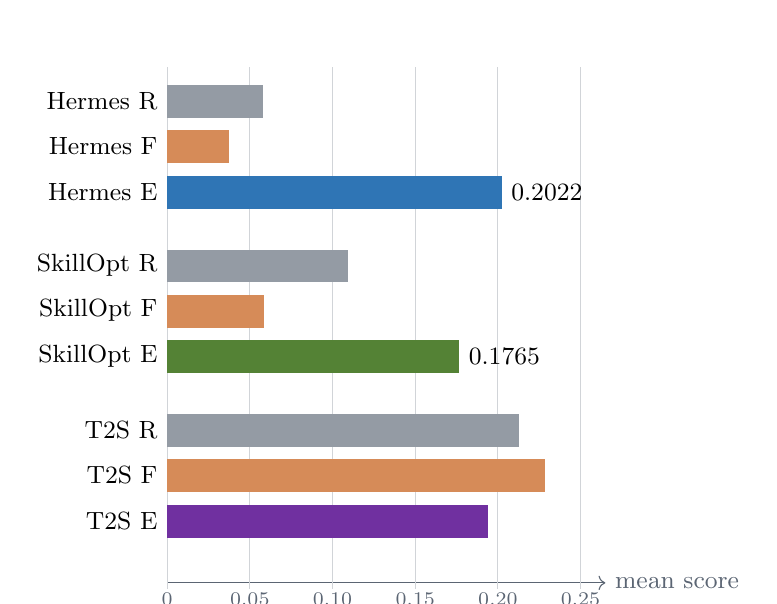
\begin{tikzpicture}[x=21cm,y=0.72cm,font=\small]
\draw[->,gray] (0,0) -- (0.265,0) node[right]{mean score};
\foreach \x in {0,0.05,0.10,0.15,0.20,0.25} {\draw[gray!28] (\x,-0.1)--(\x,9.1); \node[below,gray] at (\x,0){\scriptsize \x};}
\node[left] at (0,8.5){Hermes R};   \fill[gray!65] (0,8.20) rectangle (0.0581,8.78);
\node[left] at (0,7.7){Hermes F};   \fill[orange!70] (0,7.40) rectangle (0.0375,7.98);
\node[left] at (0,6.9){Hermes E};   \fill[blue] (0,6.60) rectangle (0.2022,7.18); \node[right] at (0.2022,6.89){0.2022};
\node[left] at (0,5.6){SkillOpt R}; \fill[gray!65] (0,5.30) rectangle (0.1096,5.88);
\node[left] at (0,4.8){SkillOpt F}; \fill[orange!70] (0,4.50) rectangle (0.0588,5.08);
\node[left] at (0,4.0){SkillOpt E}; \fill[green] (0,3.70) rectangle (0.1765,4.28); \node[right] at (0.1765,3.99){0.1765};
\node[left] at (0,2.7){T2S R};      \fill[gray!65] (0,2.40) rectangle (0.2125,2.98);
\node[left] at (0,1.9){T2S F};      \fill[orange!70] (0,1.60) rectangle (0.2287,2.18);
\node[left] at (0,1.1){T2S E};      \fill[purple] (0,0.80) rectangle (0.1941,1.38);
\end{tikzpicture}
\end{center}

Hermes 的 evolving 分数约为 reset 的 3.48 倍，并且同时高于 frozen，说明其收益不能只用工作区连续性解释。SkillOpt 也呈现同方向结果，但幅度小于 Hermes。Trace2Skill 则相反：reset 和 frozen 本身较高，evolving 没有进一步提升，说明它的基础执行并非完全失效，问题集中在学习更新是否把有效轨迹转化为可复用技能。

\subsection{按 Stream 分解增益}

\begin{center}
\scriptsize
\renewcommand{\arraystretch}{1.22}
\setlength{\tabcolsep}{4.6pt}
\begin{tabular}{llrrrrr}
\toprule
Agent & Stream & Reset & Frozen & Evolving & $\Delta$E-R & $\Delta$E-F \\
\midrule
Hermes & AIRS SICK & 0.5000 & 0.0000 & 0.2500 & -0.2500 & +0.2500 \\
Hermes & MLGym Titanic & 0.0000 & 0.0000 & 1.0000 & +1.0000 & +1.0000 \\
Hermes & SkillLearn Stock & 0.0675 & 0.0525 & 0.1425 & +0.0750 & +0.0900 \\
Hermes & SkillsBench D3 & 0.0300 & 0.0675 & 0.1500 & +0.1200 & +0.0825 \\
Hermes & Tau2 Telecom & 0.0000 & 0.0075 & 0.1450 & +0.1450 & +0.1375 \\
\midrule
SkillOpt & AIRS SICK & 0.2500 & 0.0000 & 0.5000 & +0.2500 & +0.5000 \\
SkillOpt & MLGym Titanic & 1.0000 & 0.0000 & 1.0000 & 0.0000 & +1.0000 \\
SkillOpt & SkillLearn Stock & 0.0525 & 0.0525 & 0.1200 & +0.0675 & +0.0675 \\
SkillOpt & SkillsBench D3 & 0.0300 & 0.0450 & 0.1500 & +0.1200 & +0.1050 \\
SkillOpt & Tau2 Telecom & 0.0400 & 0.1025 & 0.0300 & -0.0100 & -0.0725 \\
\midrule
Trace2Skill & AIRS SICK & 0.7500 & 0.5000 & 0.2500 & -0.5000 & -0.2500 \\
Trace2Skill & MLGym Titanic & 1.0000 & 1.0000 & 1.0000 & 0.0000 & 0.0000 \\
Trace2Skill & SkillLearn Stock & 0.1575 & 0.1525 & 0.1500 & -0.0075 & -0.0025 \\
Trace2Skill & SkillsBench D3 & 0.1250 & 0.1700 & 0.1625 & +0.0375 & -0.0075 \\
Trace2Skill & Tau2 Telecom & 0.0900 & 0.1550 & 0.0975 & +0.0075 & -0.0575 \\
\bottomrule
\end{tabular}
\end{center}

Hermes 的正增益覆盖 Titanic、两条 D3/Stock 可视化流和 Telecom，说明其学习收益不是由单一任务偶然拉动；唯一相对 reset 的负项是只有 2 turns 的 AIRS。SkillOpt 在 AIRS、Stock 和 D3 上为正，但 Telecom 为负，表现出明显的任务依赖。Trace2Skill 只有 D3 相对 reset 小幅提高，且相对 frozen 仍为负；其负增益主要来自 AIRS 和 Telecom，而不是某个 evaluator 故障。

\subsection{按 Sequence Role 分解}

\begin{center}
\scriptsize
\renewcommand{\arraystretch}{1.2}
\begin{tabular}{llrrr}
\toprule
Agent & 条件顺序 & Learning & Application & Probe \\
\midrule
Hermes & R / F / E & 0.130 / 0.030 / \textbf{0.315} & 0.030 / 0.045 / \textbf{0.138} & 0.081 / 0.025 / \textbf{0.283} \\
SkillOpt & R / F / E & 0.330 / 0.015 / \textbf{0.390} & 0.044 / 0.074 / \textbf{0.094} & 0.133 / 0.050 / \textbf{0.242} \\
Trace2Skill & R / F / E & \textbf{0.470} / 0.380 / 0.290 & 0.134 / \textbf{0.151} / 0.130 & 0.244 / \textbf{0.317} / 0.283 \\
\bottomrule
\end{tabular}
\end{center}

Hermes 和 SkillOpt 的 evolving 条件在 learning、application、probe 三类 role 上都高于 reset，尤其 probe 提升最能支持“学习后迁移”的解释。Trace2Skill 的 evolving 在三类 role 上均未超过对应的最佳 control，因此当前结果不能被包装成正向自进化。

\subsection{探针成本与结果可信度}

\begin{center}
\renewcommand{\arraystretch}{1.2}
\begin{tabular}{llrrrr}
\toprule
Condition & Agent & Turns & Passed & Tokens & Tokens/turn \\
\midrule
Reset & Hermes & 34 & 0 & 1.91M & 56,241 \\
Reset & SkillOpt & 34 & 2 & 3.30M & 97,199 \\
Reset & Trace2Skill & 34 & 3 & 13.65M & 401,324 \\
Frozen & Hermes & 34 & 0 & 3.01M & 88,602 \\
Frozen & SkillOpt & 34 & 0 & 6.86M & 201,776 \\
Frozen & Trace2Skill & 34 & 2 & 20.69M & 608,604 \\
\bottomrule
\end{tabular}
\end{center}

新增 control 运行完成 30/30 jobs、204/204 turns，审计确认 204 条原生 verifier evidence 完整；794 个 usage 字段中的 reasoning tokens 全为 0；204 个 evolution barrier 均按条件跳过且学习状态 hash 不变；最终报告中没有 framework error 或 cleanup error。一次模型请求超时从 post-agent checkpoint 精确恢复，前 4 个 turns 和第 5 个 turn 已付费回复没有重跑。

需要同时保留两个统计边界。第一，当前匹配探针只有 34 turns/condition/Agent，且各 stream 最长 10 turns，因此不满足至少两个 10-turn bin 的正式 learning-curve 趋势声明；本报告只解释条件均值和匹配增益。第二，evolving 与 control 来自不同时间的真实 API 运行，尽管模型、任务、评测器和 turn identity 一致，仍可能含有模型采样与服务波动；下一步应补充多随机种子重复。

\section{综合结论}

\begin{itemize}
  \item \textbf{任务能力与自进化能力需要分开排序。} 全量 L1 上 SkillOpt 最优，L2 上 Hermes 最优；但 L2 探针中 Hermes 的自进化增益最大。
  \item \textbf{Hermes 当前最接近“学习提高后续表现”。} 它对 reset 和 frozen 都有稳定正增益，且覆盖 application 与 probe role；代价是全量 L2 token/turn 最高。
  \item \textbf{SkillOpt 是更高效的折中方案。} 它在 L1/L2 全量矩阵中 token 效率最好，L2 探针也有正增益，但 Telecom 的负项提示技能更新具有任务依赖。
  \item \textbf{Trace2Skill 的瓶颈是演化收益而非单次能力。} 它在 reset/frozen 下并不总是差，甚至 control 均值最高；真正问题是 evolving 没有超过 control，并伴随最高调用放大。
  \item \textbf{当前结果已经可审计。} 全量矩阵有 87/87 jobs、1,671/1,671 turns；L1 采用 checkpoint 上的确定性原生复验修复历史权限污染，L2 原生证据 402/402；探针另有 204/204 条原生证据与完整 trace。
\end{itemize}

下一阶段最有价值的实验不是继续扩大单次长流，而是对 5-stream 探针做多随机种子重复，并针对 Trace2Skill 分别消融 skill 检索、MAP/REDUCE 聚合与 APPLY/VERIFY 阶段。这样可以判断负增益究竟来自技能质量、检索命中还是多阶段更新噪声。

\section{结果与证据位置}

\begin{itemize}
  \item 全量矩阵最终审计：\code{runs/mx24/final\_audit\_server\_20260907/matrix.json}
  \item L2 control 最终审计：\code{runs/mx25/l2-controls/final\_audit.json}
  \item 三条件正式探针聚合：\code{runs/mx25/l2-controls/formal\_probe\_matrix.json}
\end{itemize}

\clearpage
\appendix
\section{Hermes 完整短流 Trace}

以下完整 7-turn / 13-interaction 真实 trace 展示 request、response、actions、工具调用、Judge、feedback、state keys 与 usage。它用于说明统一生命周期，不参与本报告矩阵聚合。

\lstset{basicstyle=\fontspec{Microsoft YaHei}\fontsize{4.6}{5.4}\selectfont,breaklines=true,breakatwhitespace=false,columns=fullflexible,keepspaces=true,frame=single,rulecolor=\color{gray!45},xleftmargin=3pt,xrightmargin=3pt}
\lstinputlisting[language={},title={Hermes L1: 7 turns / 13 interactions}]{docs/report_assets/final_matrix_analysis_20260911/hermes_l1_trace.txt}

\clearpage
\section{SkillOpt 完整短流 Trace}

以下完整 5-turn 真实记录覆盖 profile fact、delayed use、config repair、JSON artifact、LLM Judge 和逐 Turn evolution evidence。

\lstinputlisting[language={},title={SkillOpt: 5 turns / 5 interactions}]{docs/report_assets/final_matrix_analysis_20260911/skillopt_trace.txt}

\clearpage
\section{Trace2Skill 完整短流 Trace}

以下完整 5-turn 真实记录保留 bash/tool calls、路径恢复、文件 observation、Judge 结果和公开 evolution 轨迹。

\lstinputlisting[language={},title={Trace2Skill: 5 turns / 6 interactions}]{docs/report_assets/final_matrix_analysis_20260911/trace2skill_trace.txt}

\end{document}
